\chapter{Анализ предметной области}
% выбор направления исследований, включающий обоснование направления исследования,
% методы решения задач и их сравнительную оценку
% описание выбранной общей методики проведения НИР;

Для начала рассмотрим игры, которые будут решаться в данной работе. Сначала даны их виды, рассмотрены проблемы связанные с ними, а затем представлены описания игр.
Все игры, рассматриваемые в работе сводятся к Марковским играм (\ref{sec:markov-games}), они подробно описаны в конце.
Таким образом, предметную область искусственного интеллекта в играх формализуется с помощью математических моделей. 
Ниже приведена формализация предметной области.

Методика выполнения НИР состоит в выявлении критериев применимости методов решения задач, а также в сравнении этих методов.

%%%%%%%%%%%%%%%%%%%%%%%%%%%%%%%%%%%%%%%%%%%%%%

\section{Виды игр}

В работе рассматриваются три вида игр. Опишем каждый их видов подробнее.

\subsection{Кооперативные игры}

В полностью кооперативных играх все агенты разделяют общую функцию наград. Такие игры так же называются MDP с несколькими агентами \newline (MMDP).
При данном условии, все Q--функции и V--функции агентов совпадают. Таким образом, оптимальная стратегия для каждого агента является совместной стратегией.
Можно использовать Q--обучение для обучения совместной стратегии. эквилибриум Нэша достигается.

Альтернативным подходом является использование функции наград для каждого агента в отдельности, награда команды определяется как среднее значение награды каждого агента.
Подобный подход подразумевает обучение агентов независимо друг от друга (decentralized MARL), а также использование протокола коммуникации между агентами.
Подразумевается, что агенты изобретут схему коммуникации (язык), которая позволит им достичь оптимальной совместной стратегии.

\subsection{Соревновательные игры}

Полностью кооперативные игры обычно моделируются как игры с нулевой сумой, то есть \( \sum_{i \in \mathcal{N}} R^i(s,a,s') = 0 \).
Большинство исследований в области соревновательных игр рассматривают среду с двумя агентами.
эквилибриум Нэша описывает стратегию оптимизирующую худшую награду в долгосрочном периоде.

\subsection{Смешанные игры}

Смешанные игры также известны как игры с общей суммой (general sum games). В таких играх сумма наград всех агентов может быть любой, как и отношения между агентами.

\section{Проблемы применимости к предметной области}

Применяя методы обучения с подкреплением к игровому искусственному интеллекту, выявляются следующие проблемы:
\begin{itemize}[label=---]
	\item комбинаторная сложность --- размер пространства действий растет экспоненциально с увеличением числа агентов;
	\item оптимизируемые величины многомерны --- эффективность обучения агентов нельзя описать одной метрикой;
	\item проблема нестабильности --- агенты, которые являются частью среды, обучаются независимо: динамика среды меняется.
	\item редкая награда --- награда может приходить только в конце матча.
\end{itemize}

\section{Рассматриваемые игры}

Рассматриваемые игры являются смешанными.
Были рассмотрены следующие игры:
\begin{itemize}[label=---]
	\item Проблемы повторяющихся матриц (Matrix Games) --- игры, награды которых описываются матрицами. Они усложнены тем, что существует локальный минимум на пути к эквилибриуму;
	\item Частицы с несколькими агентами (MPE) \ref{fig:mpe} --- несколько двумерных проблем навигации: Штурман-Искатель, Разносчик, Советчик, \newline Жертва-Хищник;
	\item StarCraft (SMAC) --- сценарий компьютерной игры StarCraft с несколькими агентами;
	\item Level Based Foraging (LBF) --- агенты должны собрать еду на карте, чтобы выжить;
	\item Robotic Warehouse (RWARE) --- агенты должны донести предметы до пункта назначения, а потом вернуться в начало.
\end{itemize}

\begin{figure}[H]
	\begin{center}
	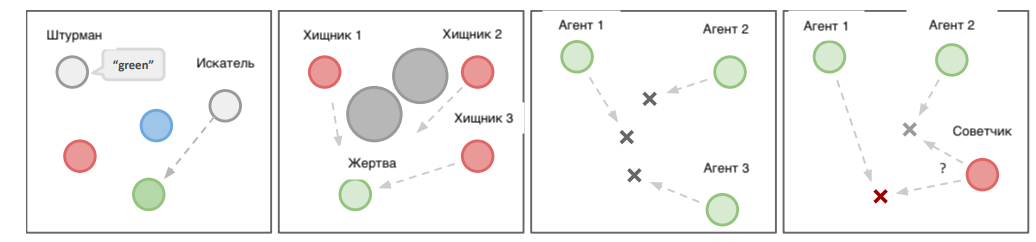
\includegraphics[pages=-, width=140mm]{./inc/img/mpe.png}
	\caption{Среды MPE, слева--направо: Штурман говорит Искателю к какой точке идти, Жертва скрывается от Хищников в серое убежище, Разносчики идут по разным местам, Советчик координирует Разносчиков.}
	\label{fig:mpe}
\end{center}
\end{figure}

Таблицы \ref{tab:games1} и \ref{tab:games2} сравнивают игры по разным критериям.

% Please add the following required packages to your document preamble:
\begin{table}[H]
	\centering
	\caption{Сравнение игр по наблюдаемости и количеству наград}
	\label{tab:games1}
	\begin{tabular}{@{}|l|l|l|@{}}
	\toprule
	Игра   & Наблюдаемость     & Кол--во наград \\ \midrule
	Матричные игры & Полная            & Много         \\
	MPE            & Полная / Неполная & Много         \\
	SMAC           & Полная / Неполная & Много         \\
	LBF            & Полная / Неполная & Крайне мало   \\
	RWARE          & Полная / Неполная & Крайне мало   \\ \bottomrule
	\end{tabular}
\end{table}

% Please add the following required packages to your document preamble:
% \usepackage{booktabs}
\begin{table}[H]
	\centering
	\caption{Сравнение игр по сложности и количеству агентов}
	\label{tab:games2}
	\begin{tabular}{@{}|l|l|l|@{}}
	\toprule
	Игра   &   \# агентов & Главная сложность             \\ \midrule
	Матричные игры &   2                   & Не оптимальный эквилибриум    \\
	MPE            &   2--3                 & Нестационарность              \\
	SMAC           &   2--10                & Большое пространство действий \\
	LBF            &   2--4                 & Координирование               \\
	RWARE          &   2--4                 & Крайне мало наград            \\ \bottomrule
	\end{tabular}
\end{table}

\section{Формализация}

Изложенные выше игры формализуются математическим языком согласно \cite{DBLP:journals/corr/abs-2011-00583} с помощью понятия Марковских игр.
Ниже представлены описания некоторых важных функций, используемых для решения игр.
Решение подразумевает поиск оптимальной стратегии. Определение оптимальной стратегии использует эти функции.

В последующих разделах под функцией будет подразумеваться нейросеть.

\subsection{Марковский процесс принятия решений} \label{sec:mdp}

Для среды с одним агентом Марковский процесс принятия решений (MDP) задается кортежем \( (\mathcal{S}, \mathcal{A}, \mathcal{P}, R, \gamma )\), элементы которого определяются следующим образом:

\begin{itemize}[label=---]
	\item \(\mathcal{S}\) --- множество состояний среды;
	\item \( \mathcal{A} \) --- множество действий агента;
	\item \( \mathcal{P}: \mathcal{S} \times \mathcal{A} \times \mathcal{S} \mapsto [0, 1] \) --- вероятность перехода из состояния \( s \in \mathcal{S} \) в состояние \( s' \in \mathcal{S} \) при выполнении действия \( a \in \mathcal{A} \);
	\item \( R: \mathcal{S} \times \mathcal{A} \times \mathcal{S} \mapsto R^1 \) --- награда за совершение действия \( a \in \mathcal{A} \) в состоянии \( s \in \mathcal{S} \) и переход в состояние \( s' \in \mathcal{S} \);  
	\item \( \gamma \in [0, 1] \) --- коэффициент дисконтирования, влияет на вероятность предпочтения немедленной награды награде в будущем.
\end{itemize}

На каждом шаге агент наблюдает состояние среды \(s_t\) в момент времени \(t\) и принимает действие \(a_t\)

Решением задачи является стратегия \( \pi \), которая определяется следующим образом\footnote{Стратегия зависит от начального состояния \(s_0\) и от предыдущих принятых действий (т. е. от самой себя). Стратегия максимизирует ожидаемую награду, которая вычисляется по формуле Беллмана.}:

\begin{equation}
	\pi(s) = \arg\max_{a \in \mathcal{A}} \mathbb{E} \left[ \sum_{t=0}^{\infty} \gamma^t R(s_t, a_t, s_{t+1}) \mid a_t \sim \pi(\cdot \mid s_t), s_0 \right].
	\label{eq:Q}
\end{equation}


Определим Q-функцию\footnote{Какую награду можно ожидать, если на шаге t выполним действие a, а дальше будем придерживаться стратегии?} и V-функцию значений\footnote{Какую награду можно ожидать, если будем придерживаться лучших действий согласно стратегии?} как:

\begin{equation}
	Q^{\pi}(s, a) = \mathbb{E} \left[ \sum_{t=0}^{\infty} \gamma^t R(s_t, a_t, s_{t+1}) \mid a_t \sim \pi(\cdot \mid s_t), s_0 = s, a_0 = a \right],
	\label{eq:V}
\end{equation}


\begin{equation}
	V^{\pi}(s) = \mathbb{E} \left[ \sum_{t=0}^{\infty} \gamma^t R(s_t, a_t, s_{t+1}) \mid a_t \sim \pi(\cdot \mid s_t), s_0 = s \right].
\end{equation}

Полным решением проблемы является оптимальная стратегия \(\pi^*\). В большинстве случаев найти оптимальную стратегию невозможно, и приближенное решение удовлетворительно. Одним из таких приближенных решений является метод итеративного улучшения стратегии (policy iteration).

\subsection{Марковские игры} \label{sec:markov-games}

Одним из обобщений Марковского процесса принятия решений (MDP) являются Марковские игры (MG).
Также используется термин стохастические игры.

Марковская игра определена кортежем \((\mathcal{N}, \mathcal{S}, \{\mathcal{A}^i\}_{i \in \mathcal{N}}, \mathcal{P}, \{R^i\}_{i \in \mathcal{N}}, \gamma)\).

Большинство определений сохраняются из Марковского процесса принятия решений (\ref{sec:mdp}), новые определения следующие:
\begin{itemize}[label=---]
	\item \(\mathcal{N}\) --- множество агентов;
	\item \(\mathcal{S}\) --- множество состояний;
	\item \(\mathcal{A}^i\) --- множество действий агента i;
	\item \(\mathcal{P}\) --- множество вероятностей перехода;
	\item \(R^i\) --- функция награды агента i.
\end{itemize}

Целью агента i является оптимизация его награды в долгосрочном периоде, путем нахождения оптимальной стратегии \(\pi^i: \mathcal{S} \mapsto \Delta (\mathcal{A}^i) \)\footnote{ \(\Delta\) означает, что пространство действий поменяется в новом состоянии.}.

В контексте нескольких агентов, многие величины становятся многомерными. Введем еще несколько определений:
\begin{itemize}[label=---]
	\item \(s = (s^1, \; \dots \;, s^n)\) --- состояния, в котором находятся агенты;
	\item \(a = (a^1, \; \dots \;, a^n)\) --- действия, принимаемые агентами в состоянии s;
	\item \( \pi : S \mapsto \Delta A \) --- совместная стратегия.
\end{itemize}

В частности, определим функцию \( V^i_{\pi^i, \pi^{-i}} \):

\begin{equation}
	V^i_{\pi^i, \pi^{-i}}(s) = \mathbb{E}_{\pi^i, \pi^{-i}} \left[ \sum_{t=0}^{\infty} \gamma^t R^i(s_t, a_t, s_{t+1}) \mid a^i_t \sim \pi^i(\cdot|s_t), s_0=s \right],
\end{equation}

где i означает множество всех агентов кроме i.

Таким образом концепт решения MG отличается от MDP тем, что оптимальная стратегия каждого агента зависит от стратегий всех остальных агентов.

Одним из решений марковских игр является эквилибриум Нэша. эквилибриум Нэша это совместная стратегия \(\pi^*=(\pi^{1,*}, \; \dots \;, \pi^{N, *})\) такая, что для каждой \(s \in \mathcal{S}\) и  \(i \in \mathcal{N}\):


\begin{equation}
	V^i_{\pi^{i, *}, \pi^{-i, *}}(s) \geq  V^i_{\pi^i, \pi^{-i, *}}(s), \; \forall  \; \pi^i.
\end{equation}

Эквилибриум Нэша характеризует точку равновесия \(\pi^*\), в которой каждому агенту не выгодно изменить свою стратегию.
Иными словами, для любого агента \(i\) стратегия \(\pi^{i, *}\) является оптимальной стратегией в условиях, когда все остальные агенты играют по стратегии \(\pi^{-i, *}\).

Доказано, что существует хотя бы один эквилибриум Нэша для Марковской игры с конечным числом состояний и конечным горизонтом (числом шагов до окончания игры).

Большинство рассматриваемых алгоритмов сходятся к точке эквилибриума Нэша.

\subsection{Описание задачи}

Задачей является поиск этой оптимальной стратегии для агента, описанной выше.

Агенту подается на вход состояние среды (той части, которую он видит), а также награда за предыдущее действие. 
На выходе агент должен выдать действие, которое он собирается совершить в данном состоянии.
Действие может выражаться дискретной величиной, например, направлением движения, или непрерывной величиной, например, углом поворота.

\begin{figure}[H]
	\label{fig:mdp}
		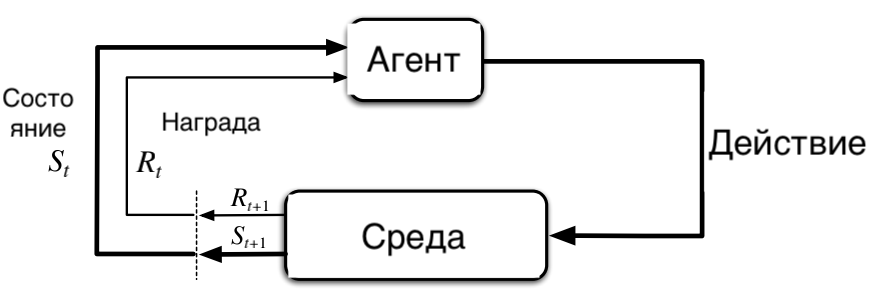
\includegraphics[width=\textwidth]{./inc/img/mdp.png}
		\caption{Марковский процесс принятия решений}
\end{figure}

Если у агентов одинаковые возможности (допустим они игроки онлайн шутера), можно использовать среднюю награду за игру, как метрику качества стратегии.
Более обобщенной метрикой служит процент побед. 

\pagebreak

Могут быть введены следующие ограничения:

\begin{itemize}[label=---]
	\item количество шагов в игре --- горизонт;
	\item смерть агента --- умершему агенту поступают в наблюдения нулевые векторы, а действия игнорируются;
	\item допустимость действия --- недопустимые дискретные действия маскируются и не могут быть выполнены;
	\item наблюдаемость среды --- агент может наблюдать лишь доступную ему часть среды;
	\item возможность коммуникации --- агенты могут или не могут обмениваться информацией.
\end{itemize}


Для недопущения действий, выражаемых векторами, существует дополнительный класс алгоритмов называющихся
безопасными алгоритмами обучения с подкреплением. Их рассмотрение выходит за рамки данной работы.

\subsection*{Вывод}

Был произведен анализ предметной области, выделены проблемы игрового искусственного интеллекта, задача формализована с использованием Марковских игр.